\documentclass[a4paper,12pt]{article}

%%% Работа с русским языком
\usepackage{cmap}					% поиск в PDF
\usepackage{mathtext} 				% русские буквы в формулах
\usepackage[T2A]{fontenc}			% кодировка
\usepackage[utf8]{inputenc}			% кодировка исходного текста
\usepackage[english,russian]{babel}	% локализация и переносы

%%% Дополнительная работа с математикой
\usepackage{amsmath,amsfonts,amssymb,amsthm,mathtools} % AMS
\usepackage{icomma} % "Умная" запятая: $0,2$ --- число, $0, 2$ --- перечисление

%% Номера формул
\mathtoolsset{showonlyrefs=true} % Показывать номера только у тех формул, на которые есть \eqref{} в тексте.
%\usepackage{leqno} % Нумерация формул слева

%% Свои команды
\DeclareMathOperator{\sgn}{\mathop{sgn}}

%% Перенос знаков в формулах (по Львовскому)
\newcommand*{\hm}[1]{#1\nobreak\discretionary{}
{\hbox{$\mathsurround=0pt #1$}}{}}

%%% Работа с картинками
\usepackage{graphicx}  % Для вставки рисунков
\graphicspath{{images/}}  % папки с картинками
\setlength\fboxsep{3pt} % Отступ рамки \fbox{} от рисунка
\setlength\fboxrule{1pt} % Толщина линий рамки \fbox{}
\usepackage{wrapfig} % Обтекание рисунков текстом

%%% Работа с таблицами
\usepackage{array,tabularx,tabulary,booktabs} % Дополнительная работа с таблицами
\usepackage{longtable}  % Длинные таблицы
\usepackage{multirow} % Слияние строк в таблице

%%% Теоремы
\theoremstyle{plain} % Это стиль по умолчанию, его можно не переопределять.
\newtheorem{theorem}{Теорема}[section]
\newtheorem{lemma}{Лемма}[section]
\newtheorem{proposition}[theorem]{Утверждение}
 
\theoremstyle{definition} % "Определение"
\newtheorem{corollary}{Следствие}[theorem]
\newtheorem{problem}{Задача}[section]
 
\theoremstyle{remark} % "Примечание"
\newtheorem*{nonum}{Решение}

%%% Программирование
\usepackage{etoolbox} % логические операторы

%%% Страница
\usepackage{extsizes} % Возможность сделать 14-й шрифт
\usepackage{geometry} % Простой способ задавать поля
	\geometry{top=25mm}
	\geometry{bottom=25mm}
	\geometry{left=35mm}
	\geometry{right=20mm}
 %
\usepackage{fancyhdr} % Колонтитулы
 	\pagestyle{fancy}
 	\renewcommand{\headrulewidth}{0mm}  % Толщина линейки, отчеркивающей верхний колонтитул
% 	\lfoot{Нижний левый}
% 	\rfoot{Нижний правый}
%	\rhead{Верхний правый}
% 	\chead{Верхний в центре}
% 	\lhead{Верхний левый}
 	% \cfoot{Нижний в центре} % По умолчанию здесь номер страницы

\usepackage{setspace} % Интерлиньяж
%\onehalfspacing % Интерлиньяж 1.5
%\doublespacing % Интерлиньяж 2
%\singlespacing % Интерлиньяж 1

\usepackage{lastpage} % Узнать, сколько всего страниц в документе.

\usepackage{soulutf8} % Модификаторы начертания

\usepackage{hyperref}
\usepackage[usenames,dvipsnames,svgnames,table,rgb]{xcolor}
\hypersetup{				% Гиперссылки
    unicode=true,           % русские буквы в раздела PDF
    pdftitle={Заголовок},   % Заголовок
    pdfauthor={Автор},      % Автор
    pdfsubject={Тема},      % Тема
    pdfcreator={Создатель}, % Создатель
    pdfproducer={Производитель}, % Производитель
    pdfkeywords={keyword1} {key2} {key3}, % Ключевые слова
    colorlinks=true,       	% false: ссылки в рамках; true: цветные ссылки
    linkcolor=blue,          % внутренние ссылки
    citecolor=purple,        % на библиографию
    filecolor=magenta,      % на файлы
    urlcolor=cyan           % на URL
}

%\renewcommand{\familydefault}{\sfdefault} % Начертание шрифта

\usepackage{multicol} % Несколько колонок

\usepackage{amsfonts} % Буквы "двойными штрихами": вещественные, натуральные...

\usepackage{indentfirst} % Красная строка

%%% Пакет для создания подписей к рисункам
\usepackage{caption}

\begin{document} % конец преамбулы, начало документа

\newpage
\thispagestyle{empty} %т.е. эта страница без колонтитулов
\begin{center}
	\textit{Федеральное государственное автономное учреждение \\
		высшего профессионального образования}
	\vspace{0.5ex}
	
	\textbf{МОСКОВСКИЙ ФИЗИКО-ТЕХНИЧЕСКИЙ ИНСТИТУТ \\ (ГОСУДАРСТВЕННЫЙ УНИВЕРСИТЕТ)}
\end{center}
\vspace{13ex}
\begin{flushright} % Выравнивание по правому краю
	\noindent % убирает "красную строку"
	\textit{Вручтель Серафима Вильямовна}
	\\
	\textit{студентка факультета инноваций}
	\\
	\textit{и высоких технологий}
	\\
	\textit{(группа 495а)}
\end{flushright}
\begin{center}
	\vspace{13ex}
%	\so{\textbf{ИНДИВИДУАЛЬНЫЙ ПРОЕКТ}} % небольшие пробелы между буквами
	\textbf{ИНДИВИДУАЛЬНЫЙ ПРОЕКТ}
	\vspace{1ex}
	
	по сложности вычислений
	
	
	на тему:
	
	\textbf{\textit{<<Теория расписаний>>}}
	
	\vfill
	Москва 2016
\end{center}


\newpage

\section{Введение}

В повседневной жизни мы часто сталкиваемся с необходимостью упорядочить какие-либо действия. \\
Формально схема процесса упоредочения выглядит следующим образом: \\
Пусть $\alpha$ "--- результат выполнения сначала задачи A, а потом задачи B, $\beta$ "--- результат выполнения этих задач в обратной последовательности. Тогда, если последствия $\alpha$ предпочтительнее последствий $\beta$ выбирается последовательность <<сначала A, потом B>>. \\
На самом деле идея решения подобных задач заключается не в том, чтобы выбрать очерёдность действий в отдельной конкретно взятой проблеме, а в том, чтобы определить общие критерии, руководствуясь которыми можно принимать подобные решения.

В данной работе будут рассмотрены примеры задач теории расписаний. Также будет доказана NP-полнота некоторых из них.

\newpage

\section{Математическая модель}

Математическая модель для самой общей задачи теории расписаний выглядит следующим образом: \\
Есть $n$ работ $\{J_1, ... J_n\}$ (система непересекающихся множеств), каждая из которых может состоять из нескольких непрерываемых операций, с различным необходимым временем на выполнение.\\
Эти работы нужно выполнить на $m$ машинах $\{M_1, ... M_m\}$, минимизируя при этом временные затраты и, возможно, другие характеристики. Каждая машина может выполнять единовременно не более одной операции.

\par\bigskip
Для каждой работы $J_i$ могут быть могут быть заданы следующие величины:\\
1) количесто операций $n_i$;\\
2) порядок машин $v_i$ "--- кортеж из $n_i$ номеров машин (каждой операции соответствует номер машины, на которой она должна быть выполнена);\\
3) время выполнения k--й операции $p_{ik}$, $k=1,...,n_i$;\\
4) вес работы $w_i$;\\
5) время поступления (время готовности) работы $r_i$ "--- самое раннее возможное время начала выполнения работы;\\
6) срок выполнения (дедлайн); $d_i$\\
7) функции стоимости $f_i: \mathbb{N} \to \mathbb{R}$, обозначающие стоимости расходов, понесённых для выполнения работы $J_i$.

\par\bigskip
Зная порядок выполнения на каждой из машин $M_k$, для каждой работы $J_i$ можно вычислить следующие величины:\\
1) $S_i$ "--- время начала выполнения работы; \\
2) $C_i$ "--- время окончания выполнения работы; \\
3) $L_i$ "--- опоздание $(L_i = C_i - d_i)$;\\
4) $T_i$ "--- медлительность $(T_i = max\{0, C_i - d_i\})$;\\
5) $U_i = 0$, если $C_i \le d_i$ и $1$, иначе.

\par\bigskip
Составление расписания означает, что для каждой работы задаётся временной участок, в течение которого она должна быть выполнена, причём это выполнение должно происходить на некоторой конкретной выбранной машине.


\newpage

\section{Общая классификация задач}
Задачи теории расписаний бывают двух видов: статческие и динамические. В статических задачах расписание составляется для изначально заданного и известного набора и количества конкретных работ. В динамических задачах новые работы поступают непрерывно, и время их появления неизвестно, его можно определить только в статистическом смысле.
Задачи теории расписаний также подразделяются согласно порядку выполнения машинами операций. Система машин может быть конвейерной (последовательность прохождения машин одинакова для каждой из работ) или со случайным порядком выполнения.

\par\bigskip
Далее для определения задачи будем использовать следующее обозначение:
\textbf{A|B|C|D}. \\
Здесь \textbf{A} определяет процесс поступления работ. Это может быть функция от времени для динамических систем или число одновременно поступивших работ для статических систем. \\
\textbf{B} характеризует количество машин в задаче. \\
\textbf{C} задаёт порядок выполнения работ машинами: F "--- система конвейерная, R "--- со случайным порядком, G "--- произвольная, I "--- параллельная (каждая работа выполняется на на отдельно взятой машине целиком, т.е. $n_i = 1$), может также быть указана какая-то дополнительная информация о выполнении работ машинами. \\
\textbf{D} определяет критерий оценки расписания.

\newpage

\section{Примеры задач из P}

\newcounter{zc}[section]

\newcommand{\z}[2]{ %Аргумент 1 - название задачи, 2 - текст задачи

\addtocounter{zc}{1}
\textbf{Задача \thesection.\arabic{zc}. #1}\\ #2

}

\z{$\mathbf{n|1|prec, r_i \ge 0|C_{max}}$}{Расшифруем формулировку: $n$ "--- количество задач, которые необходимо решить (имеется в виду, что это количество может быть произвольным);\\ 
задачи решаются на единственной машине; \\
запись $prec$ означает, что задачи упорядочены: работа $J_i$ предшествует работе $J_j$ ($J_i < J_j$), то есть $C_i \le S_j$ "--- выполнение работы $j$ должно начинаться не раньше, чем закончится выполнение работы $i$;\\
$r_i \ge 0$ "--- время поступления работ может быть различным (система динамическая), буква F, R, G или I не указана, так как в системе есть только одна машина;\\
в качестве критерия "--- значения, которое необходимо минимизировать, берётся $max_i\{C_i\}$, то есть хочется минимизировать общее время выполнения работ.\\
Известно, что эту задачу можно выполнить за время $O(n^2)$ (см. \cite{lenstra}).}

\par\bigskip
\z{$\mathbf{n|1|C_i \le d_i|\Sigma C_i}$}{Произвольное количество работ выполняется на одной машине. Каждая работа должна быть выполнена до некоторого фиксированного времени - дедлайна. При этом необходмо минимизировать сумму времён окончания работ.\\
Эту задачу можно выполнить за время $O(n \log{n})$. (см. \cite{lenstra})}

\par\bigskip
\z{$\mathbf{n|2|F,}$ \textit{no wait}$\mathbf{|C_{max}}$}{Произвольное количество работ выполняется на двух машинах. Система конвейерная. Запись <<\textit{no wait}>> означает, что в процессе выполнения работы не бывает простоя ($C_i = S_i + \Sigma_k p_{ik}$). Минимизируем общее время выполнения работ.\\
Задача решается за время $O(n^2)$ (см. \cite{lenstra})}

\par\bigskip
\z{$\mathbf{2|m|G|C_{max}}$}{2 работы необходимо выполнить на некотором количестве машин. Для каждой из работ последовательность выполнения операций на машинах может отличаться, то есть она не фиксируется. Хочется минимизировать общее время выполнения работ.\\
Эту задачу можно решить за время $O(m^2)$ (см. \cite{lenstra}).}

\par\bigskip
\z{$\mathbf{n|m|I|\Sigma C_i}$}{$n$ работ нужно выполнить на $m$ машинах. Каждая работа выполняется на одной конкретно взятой машине. При этом необходимо минимизировать сумму времён окончаний работ.\\
Существует алгоритм, решающий эту задачу за время $O(n \log{n})$ (см. \cite{lenstra}).}

\par\bigskip
\z{$\mathbf{n|m|I,}$ \textit{tree}, $\mathbf{p_i = 1|C_{max}}$}{$n$ работ нужно выполнить на $m$ машинах. Каждая работа выполняется на одной конкретно взятой машине. Время, необходимое для выполнения каждой из работ, совпадает. Запись <<\textit{tree}>> означает, что работы зависят друг от друга, таким образом, что можно построить граф зависимостей работ друг от друга, представляющий собой множество ориентированных деревьев, где входная или выходная вершина общая для всех деревьев. При этом необходисо минимизировать общее время выполнения.
Данная задача решается за линейное от количества работ время: $O(n)$ (см. \cite{lenstra}).}

\newpage

\section{Примеры задач из NP}

\setcounter{zc}{0}

\begin{theorem}
	Задача о рюкзаке $(Knapsack)$ сводится к следующим задачам теории расписаний:\\
	(1) $n|2|G, \, n_i \le 3|C_{max}$;\\
	(2) $n|3|G, \, n_i \le 2|C_{max}$;\\
	(3) $n|3|F|C_{max}$;\\
	(4) $n|2|F, \, r_i \ge 0|C_{max}$;\\
	(5) $n|2|F|L_{max}$;\\
	(6) $n|2|F, tree|C_{max}$;\\
	(7) $n|1|r_i \ge 0|L_{max}$;\\
	(8) $n|1||\Sigma w_i U_i$;\\
	(9) $n|1||\Sigma w_i T_i$;\\
	(10) $n|1|C_i \le d_i|\Sigma w_i C_i$;\\
\end{theorem}
\begin{proof}[Доказательство]
	Задача о рюкзаке $(Knapsack)$ формулируется следующим образом: 
	$Knapsack = \{(a_1, ..., a_t, b)| \exists \, S \subset T=\{1,...t\}: \; \Sigma_{i \in S}a_i = b\}$. Доказательство NP-полноты этой задачи см. в \cite{karp}.\\
	Обозначим $A = \Sigma_{i \in T}a_i$. Можем считать, что $0 < b < A$.
	
	\par\bigskip
	(1) $Knapsack \le_p n|2|G, \, n_i \le 3|C_{max}$.\\
	Пусть дана задача о рюкзаке. Тогда пусть\\
	$n = t + 1$ "--- число работ;\\
	$v_i = (M_1), \; p_{i1} = a_i \; \forall i \in T$ "--- все работы с индексами из T должны быть выполены на первой машине, каждая из них состоит из одной операции, время выполнения работы с индексом $i$ равно числу $a_i$;\\
	для работы с индексом n: $v_n = (M_2, M_1, M_2), \; p_{n1} = b, \; p_{n2} = 1, \; p_{n3} = A - b$ (она состоит из трёх операций);\\
	$y = A + 1$.\\
	Если задача о рюкзаке имеет решение, то существует расписание, в котором $C_{max} = y$ (см Рис. \ref{fig_1})\\
	Если у задачи о рюкзаке нет решения, то $\Sigma_{i \in S}a_i - b = c \ne 0 \: \forall \, S \subset T$, и работы выполняются на машине $M_1$ в следующем порядке: $(\{J_i| i \in S\}, J_n, \{J_j| j \in T-S\})$, так что,\\
	если $c > 0$, то $C_{max} \ge \Sigma_{i \in S}p_{i1} + p_{n2} + p_{n3} = A + c + 1 > y$,\\
	если $c < 0$, то $C_{max} \ge p_{n1} + p_{n2} + \Sigma_{i \in T-S}p_{i1} = A - c + 1 > y$.\\
	То есть задача о рюкзаке имеет решение тогда и только тогда, когда задача теории расписаний $n|2|G, \, n_i \le 3|C_{max}$ также имеет решение с $C_{max} \le y$.
	\begin{figure}[h!]
		\begin{center}
			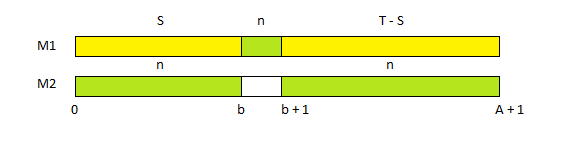
\includegraphics[scale=0.65]{pic_1.png}
			\caption[]{}
			\label{fig_1}
		\end{center}
	\end{figure}
	
	\par\bigskip
	(2) $Knapsack \le_p n|3|G, \, n_i \le 2|C_{max}$.\\
	Дана задача о рюкзаке. Тогда пусть\\
	$n = t + 2$,\\
	$v_i = (M_1, M_3), \; p_{i1} = p_{i2} = a_i \; \forall i \in T$ "--- первая операция работы $i$ выполняется на машине номер 1, вторая "--- на машине номер 3, каждая из них занимает $a_i$ времени.\\
	$v_{n-1} = (M_1, M_2), \; p_{(n-1)1} = b, \; p_{(n-1)2} = 2(A-b)$.\\
	$v_n = (M_2, M_3), \; p_{n1} = 2b, \; p_{n2} = A - b$.\\
	$y = 2A$.\\
	Если задача о рюкзаке имеет решение, то существует соответствующая задача о расписании с указанными параметрами и $C_{max} = y$ (см Рис. \ref{fig_2}).\\
	Если задача о рюкзаке не имеет решения, то $\Sigma_{i \in S}a_i - b = c \ne 0 \: \forall \, S \subset T$. Тогда на первой машине выполняются следующие работы: $(\{J_i| i \in S\}, J_{n-1}, \{J_j| j \in T-S\})$, так что\\
	если $c > 0$, то $C_{max} \ge \Sigma{i \in S}p_{i1} + p_{(n-1)1} + p_{(n-1)2} = 2A + c > y$,\\
	если $c < 0$, то $C_{max} \ge \min{\Sigma_{i \in S}p_{i1} + p_{(n-1)1} + 1, p_{n1}} + p_{n2} + \Sigma_{i \in T-S}p_{i2} = 2A + 1 > y$.\\
	То есть задача о рюкзаке имеет решение тогда и только тогда, когда построенная задача теории расписаний имеет решение.
	\begin{figure}[h!]
		\begin{center}
			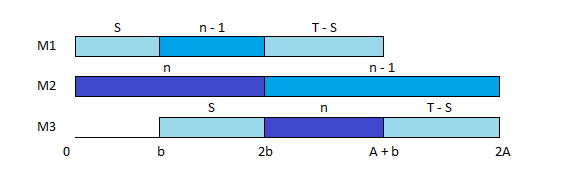
\includegraphics[scale=0.65]{pic_2.png}
			\caption[]{}
			\label{fig_2}
		\end{center}
	\end{figure}
	
	\par\bigskip
	(3) $Knapsack \le_p n|3|F|C_{max}$.\\
	Сведём задачу о рюкзаке к данной задаче теории расписаний следующим образом:\\
	$n = t + 1$ "--- количество работ,\\
	$p_{i1} = 1, \; p_{i2} = ta_i, \; p_{i3} = 1 \; \forall \, i \in T,\\
	p_{n1} = tb, \; p_{n2} = 1, \; p_{n3} = t(A - b)$. В каждой работе 3 операции.\\
	$y = t(A + 1) + 1$.\\
	Если $Knapsack$ имеет решение, то имеет решение построенная задача теории расписаний с $C_{max} = y$ (см Рис. \ref{fig_3}).
	\begin{figure}[h!]
		\begin{center}
			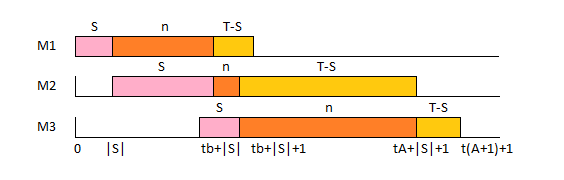
\includegraphics[scale=0.65]{pic_3.png}
			\caption[]{}
			\label{fig_3}
		\end{center}
	\end{figure}
	Если $Knapsack$ не имеет решения, то $\Sigma_{i \in S}a_i - b = c \ne 0 \: \forall \, S \subset T$. Тогда имеем порядок выполнения работ: $(\{J_i| i \in S\}, J_n, \{J_j| j \in T-S\})$, так что\\
	если $c > 0$, то $C_{max} > \Sigma{i \in S}p_{i2} + p_{n2} + p_{n3} = t(A + c) + 1 \ge y$,\\
	если $c < 0$, то $C_{max} > p_{n1} + p_{n2} + \Sigma_{i \in T-S}p_{i2} = t(A - c) + 1 \ge y$.\\
	
	\par\bigskip
	(4) $Knapsack \le_p n|2|F, \, r_i \ge 0|C_{max}$.\\
	$n = t + 1$.\\
	$r_i = 0, \; p_{i1} = ta_i, \; p_{i2} = 1 \; \forall \, i \in T$.\\
	$r_n = {tb}, \; p_{n1} = 1, \; p_{n2} = t(A-b)$.\\
	$y=t(A + 1)$.\\
	Дальнейшее сведение аналогично пункту (3).
	
	\par\bigskip
	(5) $Knapsack \le_p n|2|F|L_{max}$.\\
	В этой задаче минимизируется максимальное опоздание, то есть число $\max\{C_i - d_i\}$.\\
	$n = t + 1$.\\
	$p_{i1} = 1, \; p_{i2} = ta_i, \; d_i = t(A + 1) \; \forall \, i \in T$.\\
	$p_{n1} = tb, \; p_{n2} = 1, \; d_n = t(b + 1)$.\\	
	$y = 0$.\\
	Дальнейшее сведение аналогично пункту (3).
	
	\par\bigskip
	(6) $Knapsack \le_p n|2|F, tree|C_{max}$.\\
	$n = t + 2$.\\
	$p_{i1} = ta_i, \; p_{i2} = 1 \; \forall \, i \in T$.\\
	$p_{(n-1)1} = 1, \; p_{(n-1)2} = tb$.\\
	$p_{n1} = 1, \; p_{n2} = t(A - b)$.\\
	$J_{n - 1} < J_n$.\\
	$y = t(A + 1) + 1$.\\
	На первой машине имеем следующий порядок выполнения работ:\\
	$(\{J_i|i \in R\}, \, J_{n - 1}, \, \{J_i|i \in S\}, \, J_n, \, \{J_i|i \in T - S - R\})$ для некоторого R. Тогда, если $R \ne 0$, то\\
	$C_{max} \ge t + p_{(n - 1)1} + p{(n - 1)2} + p_{n1} + p_{n2} = A(t + 1) + 2 > y$.\\
	Тогда получаем, что $Knapsack$ имеет решение тогда и только тогда, когда предложенная задача теории расписаний имеет решение.
	
	\par\bigskip
	(7) $Knapsack \le_p n|1|r_i \ge 0|L_{max}$.\\
	В этой задаче выполнение происходит только на одной машине. Пусть\\
	$n = t + 1$;\\
	$r_i = 0, \; p_i = a_i, \; d_i = A + 1 \; \forall \, i \in T$;\\
	$r_n = b, \; p_n = 1, \; d_n = b + 1$;\\
	$y = 0$.\\
	Остальное сведение аналогично пункту (1), (см Рис. \ref{fig_4}).
	\begin{figure}[h!]
		\begin{center}
			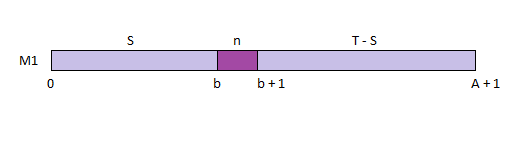
\includegraphics[scale=0.65]{pic_4.png}
			\caption[]{}
			\label{fig_4}
		\end{center}
	\end{figure}
	
	\par\bigskip
	(8) $Knapsack \le_p n|1||\Sigma w_i U_i$.\\
	$n = t$.\\
	$p_i = w_i = a_i, \; d_i = b \; \forall \, i \in T$.\\
	$y = A - b$.\\
	Тогда задача о рюкзаке имеет решение тогда и только тогда, когда приведённая задача теории расписаний имеет решение (см Рис. \ref{fig_5}).
	\begin{figure}[h!]
		\begin{center}
			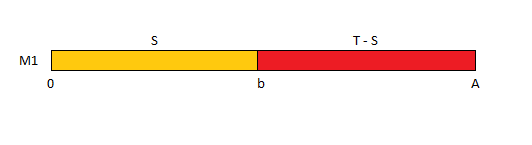
\includegraphics[scale=0.65]{pic_5.png}
			\caption[]{}
			\label{fig_5}
		\end{center}
	\end{figure}
	
	\par\bigskip
	(9) $Knapsack \le_p n|1||\Sigma w_i T_i$.\\
	$n = t + 1$.\\
	$p_i = w_i = a_i, \; d_i = 0 \; \forall \, i \in T$.\\
	$p_n = 1, \; w_n = 2, \; d_n = b + 1$.\\
	$y = \Sigma_{1 \le i \le j \le t}a_i a_j + A - b$.\\
	(См Рис \ref{fig_4}). Имеем порядок выполнения работ: $(\{J_i|i \in S\}, \; J_n, \; \{J_i|i \in T - S\})$, что $\Sigma_{i \in S}a_i - b = L_n$.\\
	Так как $p_i = w_i$ и $d_i = 0 \; \forall \, i \in T$ число $\Sigma w_i T_i$ не зависит от от порядка $S$ и $T - S$, то имеем следующее:\\
	$\Sigma w_i T_i = \Sigma_{i \in T}a_i C_i + 2 T_n = \Sigma_{1 \le i \le j \le t}a_i a_j  + \Sigma_{i \in T - S}a_i + 2\max\{0, L_n\} = y + |L_n| \ge y$.\\
	Откуда следует эквивалентность задач.
	
	\par\bigskip
	(10) $Knapsack \le_p n|1|C_i \le d_i|\Sigma w_i C_i$.\\
	$n = t + 1$.\\
	$p_i = w_i = a_i, \; d_i = A + 1 \; \forall \, i \in T$.\\
	$p_n = 1, \; w_n = 0, \; d_n = b + 1$.\\
	$y = \Sigma_{1 \le i \le j \le t}a_i a_j + A - b$.\\
	(См пункт (9) и Рис \ref{fig_4}).
	
\end{proof}

Из теоремы следует, что приведённые задачи теории расписаний являются NP-полными.

\par\bigskip

Рассмотрим следующую задачу.

\par\bigskip
\z{На выполнение каждой из работ требуется одинаковое время.}{Пусть задано множество $S$ из $n$ работ, порядок $\prec$ на $S$, весовая функция $W$, $k$ машин и ограничение на время $t$. Спрашивается, существует ли такая всюду определённая функция $f: S \to \{0, 1, ..., t - 1\}$, что выполнены следующие условия:\\
1) если $J_1 \prec J_2$, то $f(J_1) + W(J_1) \le f(J_2)$ (т.е. выполнение работы $J_1$ начнётся не раньше, чем закончится выполнение работы $J_2$);\\
2) для каждой работы $J \in S$: $f(J) + W(J) \le t$ (т.е все работы будут выполнены в отведённое время);\\
3) $\forall \, i \in \{0, ..., t\}$ есть максимум $k$ работ $J$, для которых $f(J) \le i < f(J) + W(J)$ (т.е. в каждый момент времени не может выполняться больше работ, чем существует машин).\\
Кроме того, $W(J) = 1 \; \forall \, J$.}

\par\bigskip

Эта задача является NP-полной, что можно доказать сведением несколько более общей задачи 5.2. к ней.

\par\bigskip

\z{На выполнение каждой из работ требуется одинаковое время, а количество рабочих машин может изменяться.}{Пусть задано множество $S$ из $n$ работ, порядок $\prec$ на $S$, ограничение на время $t$, а также последовательность целых чисел $c_0, \, c_1, \,..., \, c_{t - 1}$, такая что $\Sigma_{i = 0}^{t - 1} = n$. Спрашивается, существует ли такая функция $f: S \to  \{0, 1, ..., t - 1\}$, что выполнено:\\
1) множество $f^{-1}(i)$ содержит ровно $c_i$ элементов;\\
2) если $J_1 \prec J_2$, то $f(J_1) < f(J_2)$.\\
(Число $c_i$ означает количество рабочих машин в момент времени $i$.)}

\par\bigskip

\begin{lemma}
	Задача 5.2. полиномиально сводится к задаче 5.1.
\end{lemma}

\begin{proof}
	Пусть дано множество $S$, порядок на $S$, ограничение на время $t$ и последовательность чисел $c_0, \, c_1, \,..., \, c_{t - 1}$ из задачи 5.2.\\
	Введём новые работы $I_{ij}$ для $i \in \{1, ..., t\}$ и $j \in \{0, ..., n - c_i\}$. Для всех работ, которые уже были в $S$ порядок сохраним, а для новых введём следующим образом: $I_{ij} \prec I_{(i + 1)k} \: \forall \, i \in \{0, ..., t - 1\}$ и произвольных $j$ и $k$.\\
	Если мы возьмём $n + 1$ машину, то получим случай задачи 5.1.\\
	Так как при любом решении ровно $n + 1 - c_i$ из новых работ должны быть выполнены в момент времени $i$, то в каждый момент времени должны быть задействованы все машины, и задача 5.1. имеет решение тогда и только тогда, когда имеет решение задача 5.2.\\
	Время, которое потребуется на добавление новых работ в худшем случае квадратично от длины входа для 5.2. Таким образом, сведение полиномиально.
\end{proof}

\par\bigskip

\begin{lemma}
	Задача 5.2. является NP-полной.
\end{lemma}

\begin{proof}
	Доказывать будем сведением задачи $3SAT$ к 5.2. Доказательство того, что задача $3SAT$ является NP-полной можно найти в \cite{cook}.\\ \\
	Задача $3SAT$ формулируется следующим образом.\\
	Пусть задано множество из $m$ переменных $x_i$ и набор множеств $\{D_1, ..., D_n\}$, где $m \le 3n$, таких что каждое множество из $D_j$ состоит ровно из трёх элементов $x_i$ или $\overline{x}_i$, называемых литералами. Спрашивается, существует ли отображение $f: \{1, 2, ..., m\} \to \{true, false\}$, такая что $\forall \, j \in \{1, ..., n\}$ либо какая-то $x_i \in D_j$, и  $f(i) = true$, либо $\overline{x}_{i} \in D_j$ и $f(i) = false$.\\
	То есть, другими словами, спрашивается, существует ли выполняющий набор для некоторой заданной в 3КНФ формулы.\\ \\
	Теперь докажем полиномиальную сводимость $3SAT$ к задаче 5.2.\\
	Пусть дана формула в 3КНФ. Построим по ней вход для задачи 5.2.\\
	Зададим множество $S$. Пусть оно содержит следующие работы:\\
	$x_{ij}$ и $\overline{x}_{ij} \; \forall \, i \in \{1, ..., m\}$ и $j \in \{0, ..., m\}$,\\
	$y_i$ и $\overline{y}_{i} \; \forall \, i \in \{1, ..., m\}$,\\
	$D{ij} \; \forall \, i \in \{1, ..., n\}$ и $j \in \{1, ..., 7\}$.\\
	Введём отношение порядка $\prec$ на $S$ следующим образом:\\
	1) $x_{ij} \prec x_{i(j + 1)}$ и $\overline{x}_{ij} \prec \overline{x}_{i(j + 1)} \; \forall \, i \in \{1, ..., m\}$ и $j \in \{0, ..., m\}$;\\
	2) $x_{i(i - 1)} \prec y_i$ и $\overline{x}_{i(i - 1)} \prec \overline{y}_i \; \forall \, i \in \{1, ..., m\}$;\\
	3) рассмотрим $D_{ij}$, пусть $a_1 a_2 a_3$ "--- двоичное представление $j$. (Заметим, что случай $a_1 = a_2 = a_3 = 0$ невозможен.) Пусть $D_i$ состоит из литералов $z_{k_1}, \, z_{k_2}, \, z_{k_3}$, где каждый из $z$ независимо от других отвечает за некоторый литерал $x$ или $\overline{x}$. Тогда для $1 \le p \le 3$ если $a_p = 1$, то пусть $z_{k_p m} \prec D_{ij}$, если $a_p = 0$, то пусть $\overline{z}_{k_p m} \prec D_{ij}$.\\
	Введём ограничение на время $t = m + 3$ и числа $c_i$ для $i \in \{0, ..., m + 2\}$. $c_i$ определим следующим образом:\\
	$c_0 = m$,\\
	$c_1 = 2m + 1$,\\
	$c_i = 2m + 2$, если $2 \le i \le m$,\\
	$c_{m + 1} = n + m + 1$,\\
	$c_{m + 2} = 6n$.\\ \\
	Теперь нужно показать, что построенная задача имеет решение тогда и только тогда, когда имеет решение соответствующая задача из $3SAT$. Интуитивная идея предстоящего доказательства следующая: мы можем считать, что литерал $x_i$ (или $\overline{x}_i$) истинен тогда и только тогда, когда работа $x_{i0}$ (или $\overline{x}_{i0}$, соответственно) выполнилась в момент времени $t = 0$. Также заметим, что существование $y$'ов и $\overline{y}$'ов даёт возможность только одной работе из $x_{i0}$ или $\overline{x}_{i0}$ выполняться в момент времени $t = 0$. Также заметим, что необходимость $n + m + 1$ работе выполняться в момент времени $t = m + 1$ эквивалентна необходимости для каждого $i$ существования только одного $j$, что работа $D_{ij}$ может выполняться в этот момент времени. Но это условие соответствует тому, что дизъюнкция элементов из $D_i$ выдаёт $true$ тогда и только тогда, когда все $x_i$ и $\overline{x}_i$, которые были выполнены в момент времени $t = 0$, также равны $true$.\\ \\
	Сначала покажем, что при любом решении построенной задачи для любого $i$ в момент времени $t = 0$ не могут быть одновременно выполнены работы $x_{i0}$ и $\overline{x}_{i0}$. Предположим, что это не так. Тогда, так как $c_0 = m$, будут такие $j$, что ни $x_{j0}$, ни $\overline{x}_{j0}$ не будут выполнены в момент времени $t = 0$. Тогда ни $y_j$, ни $\overline{y}_j$ не смогут быть выполнены к моменту времени $t = j$, так как выполнению $y_j$ должно предшествовать выполнение $x_{j0}, \, x_{j1}, ..., \, x_{j(j - 1)}$, где каждая из работ также должна выполняться раньше другой. Таким образом, общее количество работ, которое сможет быть выполнено к моменту времени $t = j$:\\
	1) максимум $m(2j + 1)$ из $x$'ов и $\overline{x}$'ов "--- $z_{i0}, \, z_{i1}, ..., \, z_{ij}$, если $z_{i0}$ была выполнена в момент времени $t = 0$ и $z_{i0}, \, z_{i1}, ..., \, z_{i(j - 1)}$, иначе,\\
	2) максимум $2(j - 1)$ из $y$'ов, а именно $y_1, \, \overline{y}_1, \, y_2, \, \overline{y}_2, ..., \, y_{j - 1}, \, \overline{y}_{j - 1}$.\\
	То есть общее количество работ, которое может быть выполнено к моменту времени $t = j$ "--- максимум $2mj + 2j + m - 2$. При этом для $1 \le j \le m$ верно следующее:
	\begin{equation}
		\Sigma_{i = 0}^j c_i = 3m + 1 + (j - 1)(2m + 2) = 2mj + 2j + m - 1
	\end{equation}
	Приходим к противоречию. Следовательно, можно заключить, что в момент времени $t = 0$ может быть выполнена только одна из работ $x_{i0}$ и $\overline{x}_{i0}$. Более того, мы можем точно определить, какие работы будут выполнены в каждый момент времени от $1$ до $m$, зная, какие из работ $x_{i0}$ и $\overline{x}_{i0}$ были выполнены в момент времени $t = 0$, так как в момент времени $t = k$ должна быть выполнена работа $z_{ik}$, если работа $z_{i0}$ была выполнена в момент времени $t = 0$ и работа $z_{i(k - 1)}$, если это не так. Кроме того, в момент времени $t = k$ должна быть выполнена работа $y_k$ (соответственно $\overline{y}_k$), если работа $x_{k0}$ (соответственно $\overline{x}_{k0}$), была выполнена в момент времени $t = 0$, и $y_{k - 1}$ (соответственно $\overline{y}_{k - 1}$), если работа $x_{k0}$ (соответственно $\overline{x}_{k0}$), была выполнена в момент времени $t = 1$.\\ \\
	В момент времени $t = m + 1$ могут быть выполнены оставшиеся $x$ и $\overline{x}$ и одна оставшаяся $y$ или $\overline{y}$. Так как $c_{m + 1} = m + n + 1$, то, если есть решение задачи, должны быть выполнены также $n$ работ типа $D$. Заметим, что для каждой пары $D_{i j_1}$ и $D_{i j_2}$, где $j_1 \ne j_2$, есть, как минимум, одно значение $k$, такое что работа $x_{km}$ предшествует работе $D_{i j_1}$, а работа $\overline{x}_{km}$ предшествует работе $D_{i j_2}$ или наоборот. Так как мы уже доказали, что в момент времени $t = m$ может быть выполнена только одна из работ $x_{km}$ и $\overline{x}_{km}$, то можем заключить, что для каждого $i$ максимум одна из работ $D_{i1}, \, D_{i2}, ..., \, D_{i7}$ может быть выполнена в момент времени $t = m + 1$.\\ \\
	Если мы присвоим переменной $x_k$ (соответственно, $\overline{x}_k$) значение $true$ тогда и только тогда, когда работа $x_{k0}$ (соответственно, $\overline{x}_{k0}$) была выполнена в момент времени $t = 0$, то одна из работ $D_{i1}, \, D_{i2}, ..., \, D_{i7}$ сможет выполниться в момент времени $t = m + 1$ тогда и только тогда $D_i$ принимает значение $true$. То есть мы можем заключить, что решение построенной задачи существует тогда и только тогда существует выполняющий набор для исходной формулы.
	
\end{proof}

\par\bigskip

\begin{theorem}
	Задача 5.1. является NP-полной.
\end{theorem}

\begin{proof}
	Из лемм 5.1 и 5.2 доказательство следует очевидным образом.
\end{proof}

\clearpage
\newpage

\section{Практические задачи}

\setcounter{zc}{0}

\z{Составление учебного расписания.}{Пусть заданы следующие множества: \\
H "--- множество учебных часов,\\
C "--- множество преподавателей,\\
T "--- множество предметов.\\
Пусть $\forall \, c \in C \: \exists$ подмножество $A(c) \subseteq H$ "--- допустимые часы для преподавателя c,\\
$\forall \, c \in C \: \exists \, A(t) \subseteq H$ "--- допустимые часы для предмета t,\\
$\forall (c, t) \in C \times T \; \exists \, R(c, t) \in \mathbb{Z_+}$ "--- требуемая нагрузка.\\
Нужно составить учебное расписание, такое что все учителя смогут читать все предметы, и при этом будут учтены ограничения на часы.\\
Эта задача является NP-полной. Её можно решить за полиномиальное время, в случае, если $\forall \, c \in C \; |A(c)| \le 2$ или если $\forall \, c \in C \; \forall \, t \in T \; A(c) = A(t) = H$.
}

\par\bigskip
\z{Планирование производства.}{Пусть заданы следующие числа:\\
$n \in \mathbb{Z_+}$ "--- число плановых периодов;\\
для каждого $i \in \{1,...,n\}$:\\
$r_i \in \mathbb{Z_+}$ "--- количество единиц товара, которые необходимо произвести (сырьё для производства имеется),\\
$c_i \in \mathbb{Z_+}$ "--- количество единиц товара, которые физически возможно выполнить на производстве за данный период,\\
$b_i \in \mathbb{Z_+}$ "--- стоимость переналадок и перенастроек, которые будет необходимо провести в данном периоде,\\
$p_i \in \mathbb{Z_+}$ "--- стоимость других затрат на производство продукции,\\
$h_i \in \mathbb{Z_+}$ "--- стоимость сырья, необходимого для производства;\\
$B \in \mathbb{Z_+}$ "--- максимальная сумма, которую можно потратить на производство.\\
Нужно найти для каждого $i$ соответствующее количество единиц товара $x_i \in \mathbb{Z_+}$ и количество сырья, которое необходимо докупить $I_i = \Sigma_{j=1}^i (x_j - r_j)$, такие что $\forall \, i \in \{1,...,n\} \; x_i \le c_i, \; I_i \ge 0,\\
\Sigma_{i=1}^n p_i x_i + h_i I_i + \Sigma_{x_i > 0} b_i \le B$.\\
Задача является NP-полной.
}

\par\bigskip
\z{Избежание тупика.}{Пусть задано $m$ процессов $\{P_1, ..., P_m\}$. Для каждого из процессов задан ориентированный ациклический граф переходов.\\
Пусть задано также состояние $S$, описывающее текущий активный узел для каждого из процессов (кортеж из $m$ элементов), а также $Q$ "--- множество ресурсов и некоторое распределение этих ресурсов.\\
Спрашивается, можно ли прийти в тупик из состояния $S$, то есть существует ли такой управляющий поток для каждого из процессов, что путём переходов по графу, распределением и перераспределением ресурсов система не будет приведена в некоторое конечное состояние.\\
Как и две предыдущие, эта задача также является NP-полной.
}

\newpage

\begin{thebibliography}{6}
%	\addcontentsline{toc}{section}{\refname} % чтобы список источников появился в оглавлении
	\bibitem[1]{bib1} Конвей Р.В., Максвелл В.Л., Миллер Л.В. Теория расписаний. Москва: Главная редакция физико-математической литературы изд-ва <<Наука>>, 1975.
	\bibitem[2]{bib2} Гэри М., Джонсон Д. Вычислительные машины и труднорешаемые задачи, М.: Мир, 1982.
	\bibitem[3]{lenstra} J.K. Lenstra, A.H.G. Rinnooy Kan, P. Brucker. Complexity of machine scheduling problems. North-Holland Publishing Company. Annals of Discrete Mathematics 1, 1977.
	\bibitem[4]{karp} R.M. Karp, Reducibility among combinatorial problems, in: R.E. Miller and J.W. Thatcher, eds., Complexity of computer computations (Plenum Press, New York, 1972) 85-103.
	\bibitem[5]{ullman} J.D. Ullman, NP-complete scheduling problems. Journal of computer and system sciences 10, 384-393 (1975)
	\bibitem[6]{cook} S.A. Cook, The complexity of theorem proving procedures, in "Proc. 3rd ACM Conference on Theory of Computing," May 1970, pp. 151-158.

\end{thebibliography}



\end{document} % конец документа

